\documentclass[a4paper, 11pt, openany, oneside, english]{book}
% \usepackage[utf8]{inputenc}
\usepackage{polyglossia}
\usepackage{fontspec}
% \usepackage[T1]{fontenc}
% \setmainlanguage{english}

%\usepackage[british,UKenglish,USenglish,english,american]{babel}
%\usepackage[a4paper]{geometry}
% \usepackage[a4paper,top=3cm,bottom=2cm,left=3cm,right=3cm,marginparwidth=1.75cm]{geometry}

% \usepackage[dvipsnames]{xcolor}
\usepackage{xcolor}
\definecolor{mygreen}{rgb}{0,0.6,0}
\definecolor{mygray}{rgb}{0.5,0.5,0.5}
\definecolor{mymauve}{rgb}{0.58,0,0.82}
\definecolor{bg}{rgb}{0.95,0.95,0.95}
%\definecolor{pink}{rgb}{1,0.75294117647058823529411764705882,0.7960784313725490196078431372549}

%% Watermark
\usepackage[printwatermark]{xwatermark}

%% Code Highlighting
\usepackage{minted}
%\usemintedstyle[c++]{monokai}
\newcommand{\inputmintedcpp}[1]{
\inputminted[style=fruity,%monokai,
             linenos=true,
             firstnumber=1,
             bgcolor=black, %pink,%bg,
             % frame=single,
]{cpp}{#1}
}
% \usepackage{listings}

%% Useful packages
\usepackage{url}
\usepackage{tikz}
% \usepackage{circuitikz}
\usepackage{siunitx}
\usepackage[autostyle=true]{csquotes}
\usepackage{subcaption}
\usepackage{mathtools}
\usepackage{graphicx}
\graphicspath{{./figures/}}

\usepackage{appendix}
% \renewcommand{\appendixpagename}{Annexes}
% \renewcommand{\appendixtocname}{Annexes}

\usepackage[colorlinks=true, allcolors=black]{hyperref}
\usepackage{cleveref}

% \newwatermark*[allpages,color=red!50,angle=54.736988270402746902813026801541,scale=3,xpos=0,ypos=0]{TOP SECRET}
\newsavebox{\mybox}
\savebox{\mybox}{\tikz[color=red,opacity=0.5]{\node{\textbf{TOP SECRET}};}}
\newwatermark*[
  allpages,
  angle=54.736988270402746902813026801541,
  scale=10,
  xpos=-35,
  ypos=35
]{\usebox{\mybox}}

%%% Use the package for UMONS cover page
% the option describe the faculty you belong to
% e.g. fpms, fs, ...
\usepackage[fpms]{umons-coverpage}

%%% Give the relevant pieces of information
% Your name
\umonsAuthor{Vincent \textsc{Stragier}, Georges \textsc{Tsolakis}}
% The main title of your thesis
\umonsTitle{Hardware and Software platforms} 
% The sub-title of your thesis
\umonsSubtitle{STM32 NUCLEO 64 F303RE TUTORIAL}
% The type of document: the reason of the thesis
\umonsDocumentType{Hardware and software project}
% Your supervisor(s)
\umonsSupervisor{Under the direction of Mr Carlos Alberto \textsc{VALDERRAMA SAKUYAMA}}
% The date (or academic year)
\umonsDate{2018-2019}

\begin{document}
\frontmatter
\umonsCoverPage
\tableofcontents
\newpage

\mainmatter
\phantomsection
\chapter*{Introduction}
\addcontentsline{toc}{chapter}{Introduction}
This project aims to produce a tutorial for the popular  processor and tool STM32. Many peripherals can interact with the STM32 platform but for this project the on board ADC was chosen.There are many variations of this  processor  available,we are using the STM32 Nucleo 64 F303RE variant.This variant includes many ADC that can be used in different modes such single-channel-single conversion mode, Multichannel-single conversion mode,Single-channel continuous conversion mode and others.The STM32 platform can transmit data with various ways.The option of interrupts or the DMA (Direct Memory Access) can be used.


\chapter{First hands on STM32 (Nucleo 64 F303RE)}
\section{With Mbed}
\paragraph{Preparation before code implementation}
Before the first implementation of an example code a few things need to be in place.


\begin{itemize}
  \item Install the latest driver (At the time of this tutorial "en.stsw-link009.zip")
  \item Create an mbed os account
  \item Add the card to your account (When the board shows as an removal device, click on the MBED.HTM file)
  
All the necessary packages can be found in the GitHub repository given with this tutorial
\end{itemize}

\paragraph{First upload - Led blink example }

In order to execute our first example using the STM nucleo board , the following steps must be completed .



\begin{itemize}
    \item Find the blink example on the STM32 page (on the MBED website) and open it in the compiler. 
    \item Compile the different scripts 
    \item Save the created binary file
    \item Load the created .bin file on the Nucleo board.
\end{itemize}
\newpage



\begin{listing}[!ht]
\inputmintedcpp{code_snippets/mbed-blink.cpp}
\caption{Mbed: Blink code\label{listing:mbed-Blink_code}}
\end{listing}

\begin{listing}[!ht]
\inputminted[style=fruity, linenos=true, bgcolor=black, firstline=62, lastline=86]{cpp}{code_snippets/ac6-blink.cpp}
\caption{AC6 and Platform IO: Blink code\label{listing:ac6_PIO-Blink_code}}
\end{listing}

\begin{figure}[!ht]
\centering
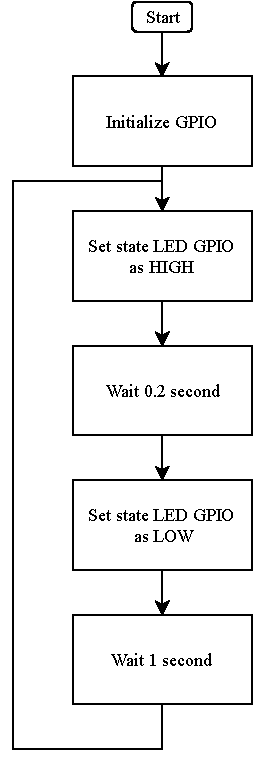
\includegraphics{mbed_blink_diag.pdf}
\caption{Block diagram for the blink code}
\end{figure}

\newpage
The previous figure show the block diagram of the blink code.As shown to the diagram the first step to executing this code is initializing the GPIO pin.After the initialization the LED GPIO pin must has a state defined as HIGH.In order to see the led light up we need to set a delay where the state of the led will remain high.After that specific delay the state drops to low and we again define a delay where the pin holds that state.

\chapter{Different ADC options}


\paragraph{Single channel-Single conversion mode}
This is the simplest form of ADC conversion,in this ADC mode a single conversion on a single channel is being done.The ADC stops after the completion of the conversion. \newline

This mode is usually implemented when we want to measure the voltage level and decide the battery level of an application.


\begin{figure}[b]
\centering
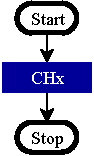
\includegraphics[width= 0.2\linewidth]{HS_STM32-single-channel-single-conversion-mode.pdf}
\caption{Block diagram for Single channel-Single conversion mode}
\end{figure}

\newpage
\paragraph{Multichannel-single conversion}



With this ADC mode a sequence of multiple channels can be configured successively  with different sampling times and different orders.

This mode can be used to make single channel measurements of multiple signals.The mode is useful for example when we want to measure the voltage level,pressure and temperature at the same time. 



\begin{figure}[b]
\centering
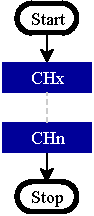
\includegraphics[width= 0.2\linewidth]{HS_STM32-single-channel_multi-single-conversion.pdf}
\caption{Block diagram for Multichannel-Single conversion mode}
\end{figure}







\newpage

\paragraph{Single-channel continuous conversion mode}
This ADC is interesting if we want the CPU load to be reduced by implementing the DMA  method in circular mode.This mode executes the  continues conversion using a single channel while allowing the ADC the work in the background without any intervention from the CPU.\\

This mode is usually implemented for the constant monitoring of the battery level in an application or for the temperature level in a device. 


\begin{figure}[b] % <3 % <3
\centering
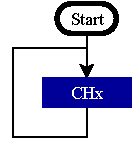
\includegraphics[width= 0.2\linewidth]{HS_STM32-single-channel_single_continuous.pdf}
\caption{Block diagram for Single-channel continuous mode}
\end{figure}

\newpage

\paragraph{Multichannel-Continuous conversion}

This mode is similar to the Multichannel-Single conversion mode.The only difference is that the conversion doesn't stop after the completion of the channel sequence but it restarts again from the first channel of the sequence.\newline

This mode can be used to monitor multiple battery or temperature levels at the same time.


\begin{figure}[b]
\centering
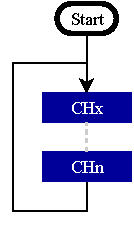
\includegraphics[width= 0.2\linewidth]{HS_STM32-single-channel_multi-single-continuous.pdf}
\caption{Block diagram for Multichannel continuous mode}
\end{figure}

\newpage
\chapter{Code explanations}

\renewcommand\listoflistingscaption{List of source codes}
\listoflistings

\end{document}